\documentclass[12pt]{report}
\usepackage[usenames,dvipsnames]{xcolor}
\usepackage{tcolorbox}
\usepackage[margin=1in]{geometry} 
\usepackage{amsmath,amsthm,amssymb}
\usepackage[english]{babel}
\usepackage[T1]{fontenc} %escribe lo del teclado
\usepackage[utf8]{inputenc} %Reconoce algunos símbolos
\usepackage{graphicx}
\usepackage{multirow}
\usepackage{wrapfig}
\usepackage{diagbox} %diagonal cells
\usepackage{dirtytalk}
\usepackage{minted}
\usepackage{booktabs}
\usepackage{import}
\usepackage{tikz}
\usepackage{pgfplots}
\usetikzlibrary{arrows.meta}
\usepackage{hyperref}
\usepackage{titlesec} % To configure subsections

\titleformat*{\subsection}{\normalsize\bfseries}
\setcounter{tocdepth}{1} % Only sections
\definecolor{bg}{RGB}{240,240,240}
\newcolumntype{Z}{>{\ttfamily}{c}<{}}


\definecolor{mintedbackground}{rgb}{0.95,0.95,0.95}

\newmintedfile[cppcode]{cpp}{
bgcolor=mintedbackground,
linenos=true,
numberblanklines=true,
numbersep=5pt,
gobble=0,
frame=leftline,
framerule=0.4pt,
framesep=2mm,
funcnamehighlighting=true,
tabsize=4,
obeytabs=false,
mathescape=false
samepage=true, %with this setting you can force the list to appear on the same page
showspaces=false,
showtabs =false,
texcl=false,
fontsize=\small
}

\setminted[cpp]{
bgcolor=mintedbackground,
linenos=true,
numberblanklines=true,
numbersep=5pt,
gobble=0,
frame=leftline,
framerule=0.4pt,
framesep=2mm,
funcnamehighlighting=true,
tabsize=4,
obeytabs=false,
mathescape=false
samepage=true, %with this setting you can force the list to appear on the same page
showspaces=false,
showtabs =false,
texcl=false,
fontsize=\small
}

\begin{document}

\begin{titlepage}
    \begin{center}
        \vspace*{1cm}
 
        \Huge
        \textbf{CP implementations}
 

 
        \vspace{1.5cm}
 
        \textbf{David del Val}
 
        \vfill
 
 
        \vspace{0.8cm}
 
 
        \Large
	\today
 
    \end{center}
\end{titlepage}

\setcounter{tocdepth}{2}
\tableofcontents 

\chapter{Graphs}

\section{Dijkstra's}
Shortest path from \texttt{orig} node to \texttt{dest} (or to every node) in a graph
that does not contain negative edges. 
It chooses the best path greedily in each iteration and, therefore, it only works
on graphs without negative weights. 
\cppcode[firstline=20]{code/graph/dijkstra.cpp}
\noindent \textbf{\boldmath Running time: $\mathcal{O}(V+E\log(E))$}
\\ {\small(V = vertices, E = edges)}

\subsection*{Observations}
\begin{itemize}
	\item If we ignore the check in line 30, we can return the distances 
		vector, which will contain the shortest distance from \texttt{dist}
		to every other node.
	\item If we are doing some kind of pruning it is imperative that we prune 
	as many branches as possible in the main loop. That is to say, we should
	introduce as many \texttt{if} statements in line 36 to make sure that we
	run the \texttt{for} loop as few times as possible. 

	An example of this approach is problem \texttt{UVA-11635}. In that problem, we
	add a lot of branches to the queue (we may run the \texttt{for} loop
	twice in some nodes) but we prune them in the main loop. Thus the 
	running time is still acceptable.

\end{itemize}

\section{Bellman Ford's}
Shortest parth from \texttt{orig} to every other node. It is slower than Dijkstra but 
it works on graphs with negative weights. 

This algorithm works by trying to relax every edge $V-1$ times. If there are no 
negative cycles, after $V-1$ iterations, we must have found the minimum distance
to every node. Therefore if after these iterations, we run another
iteration and the distance to a node decreases, we must have a negative cycle.

\cppcode[firstline=20]{code/graph/bellman_ford.cpp}
\noindent \textbf{\boldmath Running time: $\mathcal{O}(VE)$}
\\ {\small(V = vertices, E = edges)}
\subsection*{Observations}
\begin{itemize}
	\item If we keep track of the distance that decrease when we check for
		a negative cycle, we will get at least one node of 
		every negative cycle present in the graph.

		We can use this, for instance, to check if we can reach a node with 
		a cost smaller than a given bound. If it is connected to a node in a 
		negative cycle, it's distance will be as small as we want it to be
		(by looping in the cycle).

		This can be seen at play in \texttt{UVA-10557}
	\item If we modify slightly the main loop, iteration $i$ will be the 
		result of considering paths of at most $i+1$ edges:
		\begin{minted}{cpp}
for (int i = 0; i < n - 1; ++i) {
        for (auto e : edges) {
            dists2[e.fi.se] = min(dists2[e.fi.se], dists[e.fi.fi] + e.se);
        }
	dists = dists2;
}
		\end{minted}
		This can be seen at play in \texttt{UVA-11280}
		

\end{itemize}	

\section{DFS}
\subsection{Articulation points and bridges}
These algorightms can be used in undirected graphs, and we
will use the following definitions:
\begin{itemize}
	\def\itemsep{0 pt}
	\item \textbf{Articulation point}. A node whose removal would increase the number
		of connected components of the graph. That  is to say
		that it \say{splits} a connected component.
	\item \textbf{Bridge}. An edge whose removal increases the number of 
		connected components in the graph.
\end{itemize}
We will use a modified version of DFS to solve this problem. We mainly introduce two new
properties for every node:
\begin{itemize}
	\def\itemsep{0 pt}
	\item \texttt{num}. Time at which the node was first explored by DFS
	\item \texttt{low}. Earliest node that can be found in the DFS spanning 
		tree that starts from this node
\end{itemize}
When we visit a node, for every edge, there are two options:
\begin{itemize}
\def \itemsep{0pt}
	\item \textbf{Tree edge}. This edge point to a node that has not been 
		discovered yet. As such we explore it (calling \texttt{dfs})
		and, we update the value of \texttt{low} for the current
		node. 

		After the update, we can now process the child since we will
		not visit it again and it's DFS tree has been fully explored

	\item \textbf{Back edge}. This edge points to a node that has already
		been visited. Therefore, it will have a relatively low 
		\texttt{num} and we use it to update the \texttt{low}
		value of the current node
\end{itemize}
\newpage
\cppcode[firstline=20]{code/graph/articulationPts.cpp}
\noindent \textbf{\boldmath Running time: $\mathcal{O}(V+E)$}
\\ {\small (V = vertices, E = edges)}
\subsubsection*{Explanation}

The first graph that we will consider is the following:
\begin{figure}[h]
\centering
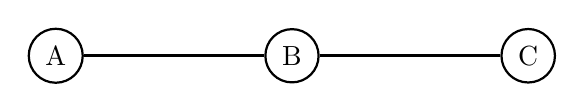
\begin{tikzpicture}
	\begin{scope}[every node/.style = {circle, thick, draw}]
		\node (A) at (0,0) {A};
		\node (B) at (3,0) {B};
		\node (C) at (6,0) {C};
	\end{scope}
	\begin{scope}[>={Stealth[black]},
			every edge/.style={draw=black, very thick}]
		\path [-] (A) edge  (B);
		\path [-] (B) edge  (C);
	\end{scope}
\end{tikzpicture}
\end{figure}
After applying DFS on $A$ we get the following DFS spanning tree.
Above every node, we have included \texttt{num / low}.
\begin{figure}[h]
\centering
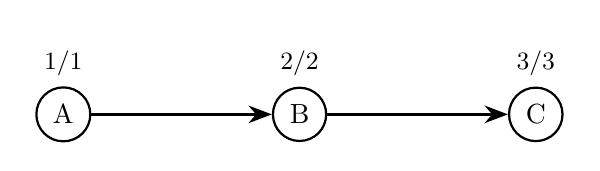
\begin{tikzpicture}
	\begin{scope}[every node/.style = {circle, thick, draw},
		every label/.append style={font = \small, yshift = -0.5 em}]
		\node[label={1/1}] (A) at (0,0) {A};
		\node[label={2/2}](B) at (3,0) {B};
		\node[label={3/3}](C) at (6,0) {C};
	\end{scope}
	\begin{scope}[>={Stealth[black]},
			every edge/.style={draw=black, very thick}]
		\path [->] (A) edge  (B);
		\path [->] (B) edge  (C);
	\end{scope}
\end{tikzpicture}
\end{figure}

This is a rather simple graph and it's only articulation point is $B$. This is because
it has a child whose \texttt{low} value is greater than or equal to $B$'s  \texttt{num}
value. Therefore, there is no connection from that child (namely $C$) to a node explored
before $B$ that does not go through $B$. 

However, we can already see that the root has to be treated as a separate case. 
The root will be an articulation point iff it has more than one child in its DFS tree. 
It is important to note that the children of the DFS tree need not be the same as the 
children of the root in the initial graph.

Let's look at another example
\begin{figure}[h]
\centering
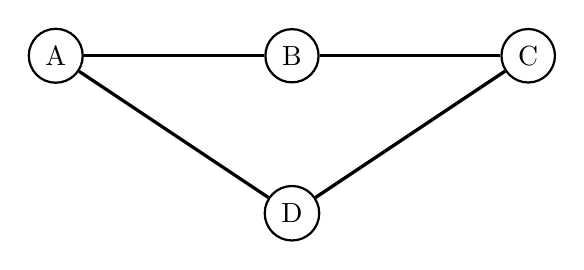
\begin{tikzpicture}
	\begin{scope}[every node/.style = {circle, thick, draw},
		every label/.append style={font = \small, yshift = -0.5 em}]
		\node (A) at (0,0) {A};
		\node (B) at (3,0) {B};
		\node (C) at (6,0) {C};
		\node (D) at (3,-2) {D};
	\end{scope}
	\begin{scope}[>={Stealth[black]},
			every edge/.style={draw=black, very thick}]
		\path [-] (A) edge  (B);
		\path [-] (B) edge  (C);
		\path [-] (C) edge  (D);
		\path [-] (D) edge  (A);
	\end{scope}
\end{tikzpicture}
\end{figure}

As before, we show the DFS spanning tree:
\begin{figure}[h!]
\centering
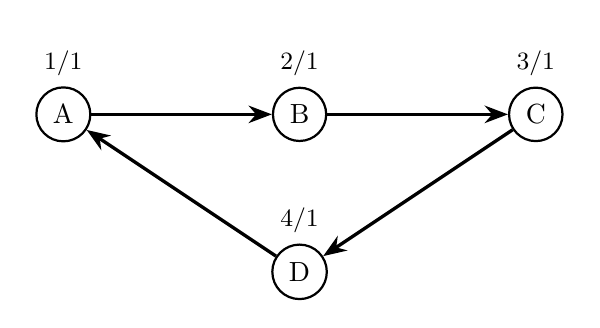
\begin{tikzpicture}
	\begin{scope}[every node/.style = {circle, thick, draw},
		every label/.append style={font = \small, yshift = -0.5 em}]
		\node [label={1/1}] (A) at (0,0) {A};
		\node [label={2/1}](B) at (3,0) {B};
		\node [label={3/1}](C) at (6,0) {C};
		\node [label={4/1}](D) at (3,-2) {D};
	\end{scope}
	\begin{scope}[>={Stealth[black]},
			every edge/.style={draw=black, very thick}]
		\path [->] (A) edge  (B);
		\path [->] (B) edge  (C);
		\path [->] (C) edge  (D);
		\path [->] (D) edge  (A);
	\end{scope}
\end{tikzpicture}
\end{figure}

Now we have no articulation point since there is no node that has a child
with a \texttt{low} greater than or equal  than the parent's \texttt{num}. 
This difference is caused by the fact that now there is an edge that makes $C$
accessible through a path that does not involve traversing $B$.

In this case, we can see how the root has only one child in the spanning tree
but two in the initial graph. This reflects the fact that those numbers need not
coincide.

Finally, the condition for a bridge is: \texttt{low[child]>num[parent]}. This is 
equivalent to  stating that the child has no other way of reaching either the
parent or a node that was explored before the parent

\subsection{Trajan's algorithm for strongly connected components}
In a directed graph, we say that a subset of vertices comprises a strongly 
connected component if every vertex is reachable from every other vertex in
this subset.

We will now present an algorithm that divides the graph into strongly
connected parts that are as large as possible. It will use some of the 
same concepts as in the previous section. 
\subsubsection*{Explanation}
The main idea is the following: if when we are done with a node, we have not been
able to reach a node that was further back, this one is the root of a SCC. 

Let's explain this reasoning with an example:

\begin{figure}[h]
\centering
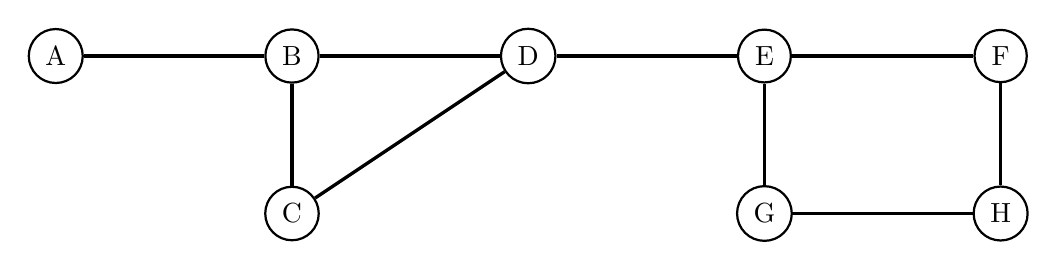
\begin{tikzpicture}
	\begin{scope}[every node/.style = {circle, thick, draw},
		every label/.append style={font = \small, yshift = -0.5 em}]
		\node (A) at (0,0) {A};
		\node (B) at (3,0) {B};
		\node (C) at (3,-2) {C};
		\node (D) at (6,0) {D};
		\node (E) at (9,0) {E};
		\node (F) at (12,0) {F};
		\node (G) at (9,-2) {G};
		\node (H) at (12,-2) {H};
	\end{scope}
	\begin{scope}[>={Stealth[black]},
			every edge/.style={draw=black, very thick}]
		\path [-] (A) edge  (B);
		\path [-] (B) edge  (C);
		\path [-] (C) edge  (D);
		\path [-] (B) edge  (D);
		\path [-] (D) edge  (E);
		\path [-] (E) edge  (F);
		\path [-] (F) edge  (H);
		\path [-] (H) edge  (G);
		\path [-] (G) edge  (E);
	\end{scope}
\end{tikzpicture}
\end{figure}
And, after running DFS, we would get the following 
spanning tree with three SCCs.

\begin{figure}[h]
\centering
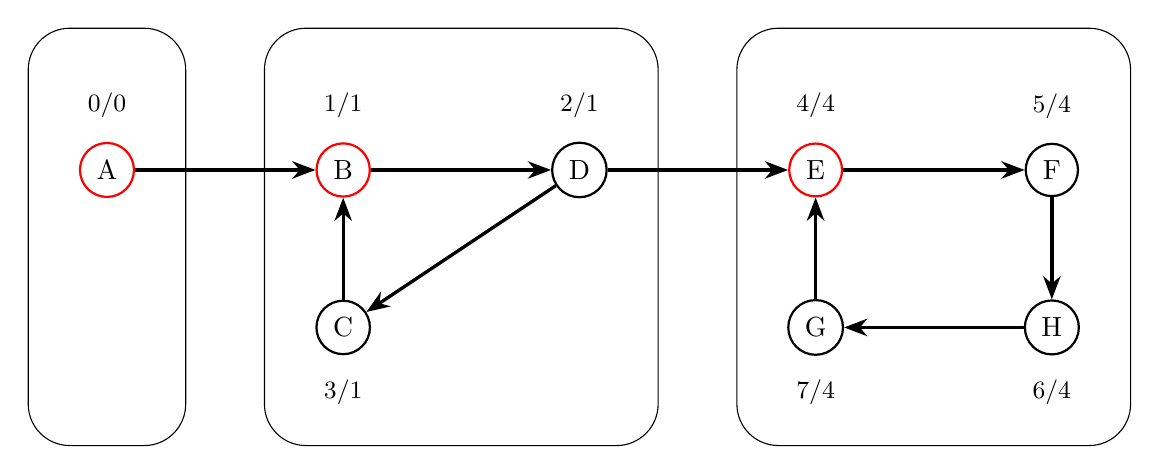
\begin{tikzpicture}
	\begin{scope}[every node/.style = {circle, thick, draw},
		every label/.append style={font = \small}]
		\node[label={0/0},draw=red] (A) at (0,0) {A};
		\node[label={1/1},draw=red] (B) at (3,0) {B};
		\node[label=below:{3/1}] (C) at (3,-2) {C};
		\node[label={2/1}] (D) at (6,0) {D};
		\node[label={4/4},draw=red] (E) at (9,0) {E};
		\node[label={5/4}] (F) at (12,0) {F};
		\node[label=below:{7/4}] (G) at (9,-2) {G};
		\node[label=below:{6/4}] (H) at (12,-2) {H};
	\end{scope}
	\begin{scope}[>={Stealth[black]},
			every edge/.style={draw=black, very thick}]
		\path [->] (A) edge  (B);
		\path [<-] (B) edge  (C);
		\path [<-] (C) edge  (D);
		\path [->] (B) edge  (D);
		\path [->] (D) edge  (E);
		\path [->] (E) edge  (F);
		\path [->] (F) edge  (H);
		\path [->] (H) edge  (G);
		\path [->] (G) edge  (E);
	\end{scope}
\draw[rounded corners=15pt] (-1,-3.5) rectangle ++(2,5.3);
\draw[rounded corners=15pt] (2,-3.5) rectangle ++(5,5.3);
\draw[rounded corners=15pt] (8,-3.5) rectangle ++(5,5.3);
\end{tikzpicture}
\end{figure}

Let's look  at the moment in which we close node $F$. As we can see the \texttt{low}
value is lower than the \texttt{num}. Therefore, there is a connection from $F$ to
another node that was visited before and it will be a part of the SCC \say{generated}
by that node.

However, when we close $E$, we can see that the \texttt{low} and the \texttt{num}
are equal. As a result, there is no way to get to a node that has a number lower than
E's through the spanning tree of $E$. Therefore, there is no way to have a bigger 
SCC that contains $E$.

To get the nodes that are part of the SCC, we need to get all the nodes in the stack before
the one that \say{generates} the SCC ($g$). This is because the stack only contains the 
nodes that belong to the spanning tree of $g$ and do not belong to any other SCC. 
Therefore, they must belong to the one generated by $g$. 

Furthermore, all those nodes will have the same \texttt{low} value since the \texttt{low}
any node with a higher value must have been processed before. Therefore, $g$ is accessible
from all those nodes and, clearly, all those nodes are accessible from $g$.
Thus, they fulfill the definition of an SCC.



\newpage
\cppcode[firstline=20]{code/graph/trajanSCC.cpp}
\noindent \textbf{\boldmath Running time: $\mathcal{O}(V+E)$}
\\ {\small (V = vertices, E = edges)}

\section{Kosaraju's}
Kosaraju's algorithm is a slightly simpler method for finding the SCC of a graph. 
On the other hand, it is also somewhat slower than Trajan's approach since it will
require running DFS on the graph twice. The algorithm follow this procedure:
\begin{enumerate}
	\item Run DFS on the graph and store the vertices in postorder in a list 
		called \texttt{postorder}.
	\item Reverse the graph
	\item Loop through the nodes in \texttt{postorder} starting from the one that 
		was closed the last. For each of them check if it has already been 
		added to a SCC (visited). If it hasn't, run DFS from that node and
		create a SCC with all the nodes that this DFS visits and hadn't been
		visited before.
\end{enumerate}
\subsubsection{Example}
Let's look at an example graph where we have run DFS starting first in node 
$A$ and, since it didn't explore the entire graph, we also run it from node $C$.
We have included the time at which each node was closed:
\begin{figure}[h]
\centering
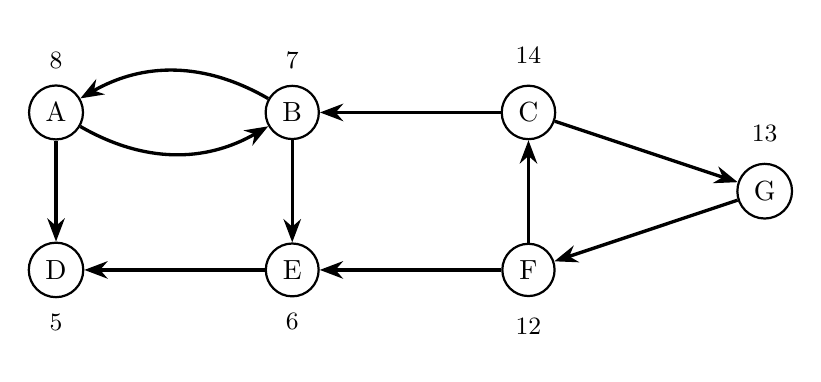
\begin{tikzpicture}
	\begin{scope}[every node/.style = {circle, thick, draw},
		every label/.append style={font = \small}]
		\node [label=8] (A) at (0,0) {A};
		\node [label=7] (B) at (3,0) {B};
		\node [label=14] (C) at (6,0) {C};
		\node [label=below:5] (D) at (0,-2) {D};
		\node [label=below:6] (E) at (3,-2) {E};
		\node [label=below:12] (F) at (6,-2) {F};
		\node [label=13] (G) at (9,-1) {G};
	\end{scope}
	\begin{scope}[>={Stealth[black]},
			every edge/.style={draw=black, very thick}]
		\path [->] (A) edge[bend right=30] (B);
		\path [->] (A) edge (D);
		\path [->] (B) edge[bend right=30] (A);
		\path [->] (B) edge (E);
		\path [->] (C) edge (B);
		\path [->] (C) edge (G);
		\path [->] (F) edge (C);
		\path [->] (F) edge (E);
		\path [->] (G) edge (F);
		\path [->] (E) edge (D);
	\end{scope}
\end{tikzpicture}
\end{figure}

Now we reverse the graph and we get the following:
\begin{figure}[h]
\centering
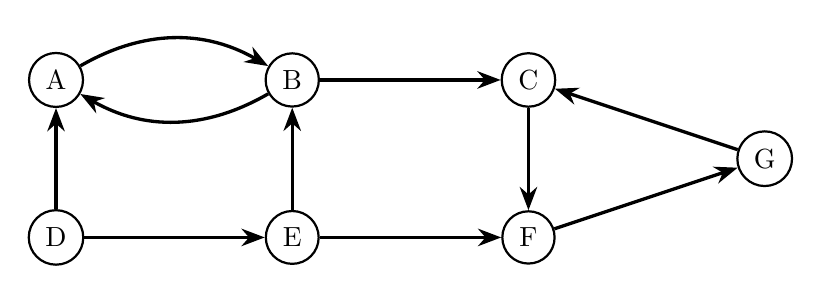
\begin{tikzpicture}
	\begin{scope}[every node/.style = {circle, thick, draw},
		every label/.append style={font = \small}]
		\node (A) at (0,0) {A};
		\node (B) at (3,0) {B};
		\node (C) at (6,0) {C};
		\node (D) at (0,-2) {D};
		\node (E) at (3,-2) {E};
		\node (F) at (6,-2) {F};
		\node (G) at (9,-1) {G};
	\end{scope}
	\begin{scope}[>={Stealth[black]},
			every edge/.style={draw=black, very thick}]
		\path [<-] (A) edge[bend right=30] (B);
		\path [<-] (A) edge (D);
		\path [<-] (B) edge[bend right=30] (A);
		\path [<-] (B) edge (E);
		\path [<-] (C) edge (B);
		\path [<-] (C) edge (G);
		\path [<-] (F) edge (C);
		\path [<-] (F) edge (E);
		\path [<-] (G) edge (F);
		\path [<-] (E) edge (D);
	\end{scope}
\end{tikzpicture}
\end{figure}


Finally, we can loop through the nodes in postorder, starting with the node
that was close the last:
\[
	\mathrm{postorder}=\{C,G,F,A,B,E,D\}
\]
\newpage
\begin{enumerate}
\def \itemsep{0pt}
	\item We run DFS on node $C$ and we get the SCC:
		\[
			s_1=\{C,F,G\}
		\]
	\item We skip nodes $G$ and $F$ in the list since they are already in
		a SCC and we run DFS on node $A$, getting the SCC:
		\[
			s_2=\{A,B\}	
		\]

	\item We skip node $B$ since it is already in a SCC and we 
		run DFS on node $E$, getting the SCC:
		\[
			s_3=\{E\}
		\]
	\item We finally run DFS on node $D$, and we get the last SCC:
		\[
			s_4=\{D\}
		\]
\end{enumerate}
Now, returning to the initial graph, we have found the following SCCs:

\begin{figure}[h]
\centering
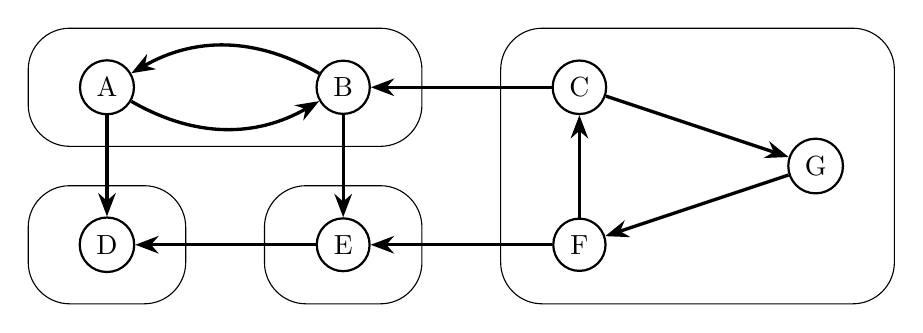
\begin{tikzpicture}
	\begin{scope}[every node/.style = {circle, thick, draw},
		every label/.append style={font = \small}]
		\node (A) at (0,0) {A};
		\node (B) at (3,0) {B};
		\node (C) at (6,0) {C};
		\node (D) at (0,-2) {D};
		\node (E) at (3,-2) {E};
		\node (F) at (6,-2) {F};
		\node (G) at (9,-1) {G};
	\end{scope}
	\begin{scope}[>={Stealth[black]},
			every edge/.style={draw=black, very thick}]
		\path [->] (A) edge[bend right=30] (B);
		\path [->] (A) edge (D);
		\path [->] (B) edge[bend right=30] (A);
		\path [->] (B) edge (E);
		\path [->] (C) edge (B);
		\path [->] (C) edge (G);
		\path [->] (F) edge (C);
		\path [->] (F) edge (E);
		\path [->] (G) edge (F);
		\path [->] (E) edge (D);
	\end{scope}
	\draw[rounded corners=15pt] (-1,-0.75) rectangle ++(5,1.5);
	\draw[rounded corners=15pt] (-1,-2.75) rectangle ++(2,1.5);
	\draw[rounded corners=15pt] (2,-2.75) rectangle ++(2,1.5);
	\draw[rounded corners=15pt] (5,-2.75) rectangle ++(5,3.5);

\end{tikzpicture}
\end{figure}
\vspace{-5 pt}
\subsubsection*{Explanation}
Let's look at why this algorithm works. 

Firstly, we have to take into account that the SCCs of a graph $G$ are preserved when 
we reverse all the edges and get $G^t$. The only relevant issue is the order in which
we process the SCCs. Let's assume we have a graph that has two SCC's:
\begin{figure}[h!]
	\centering
	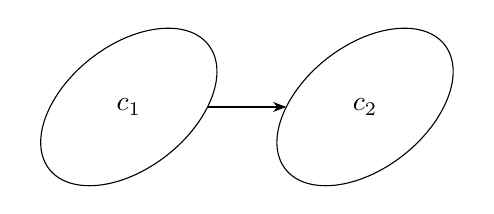
\begin{tikzpicture}
	\path[draw] plot [smooth cycle,tension=1]  coordinates 
		{(0,0) (1.5,1) (2,0) (0.5,-1)};
	\node (p1) at (1,0){$c_1$};
	
	\path[draw] plot [smooth cycle,tension=1]  coordinates 
		{(3,0) (4.5,1) (5,0) (3.5,-1)};
	\node (p1) at (4,0){$c_2$};

	\begin{scope}[>={Stealth[black]},
			every edge/.style={draw=black}]
		\path[->, ] (2,0) edge (3,0);
	\end{scope}

	\end{tikzpicture}
\end{figure}
We have three options:
\begin{itemize}
	\def\itemsep{0pt}
	\item \emph{They are not connected}. In this case, it does not matter
		whether we explore one or the other first since DFS will not 
		\say{leak} from one of them to the other
	\item \emph{They are connected only in one direction}. This is 
		the case that the figure shows and it is the most important one.
		If we explore $c_2$ before exploring $c_1$, DFS will first
		explore the entirety of $c_2$ and then, when it is exploring
		$c_1$ it will not \say{leak} to $c_2$ because those nodes are already
		marked as visited.
	\item \emph{They are connected in both directions}. This can never happen
		since, if they were to be connected bidirectionally, they would 
		form a single SCC, not two.
\end{itemize}
\newpage
Therefore, the correctness of this algorithm simply depends on exploring the SCCs in the 
right order.

Let's demonstrate the following claim: 
\vspace{-5pt}
\begin{center}
	\itshape
	In the previous setting, the maximum closing time of the nodes in $c_1$ will
	be greater than the maximum closing time of the nodes in $c_2$
\end{center}
We just have to distinguish two cases:
\begin{itemize}
	\item
	If we started exploring $c_2$ before $c_1$, there is no way to get to $c_1$ from
	$c_2$. Therefore, we will start exploring $c_1$ when we have already closed $c_2$,
	which means that all nodes in $c_2$ will be closed before the nodes in $c_1$
	are even \say{opened}.
	\item
	If we started exploring $c_1$ before $c_2$, at some point, DFS will leak to 
	$c_2$ and it will explore it entirely before returning to $c_1$. Therefore,
	the closing time of every node in $c_2$ will be lower than the closing time
	of the node where DFS was started in $c_1$.
\end{itemize}
This completes the proof of that statement. Let's now apply it to check the correctness 
of this algorithm using induction. 

\begin{itemize}
	\item \textit{Base case:}

After reversing the graph, we start with the node that was closed the last ($a$). Let's call
it's SCC $s_1$. Let's assume that there is an edge from $s_1$ to another SCC ($s_\alpha$) in
$G^t$, which would make DFS leak to that SCC. However, if that was the case, there
would be an edge from $s_\alpha$ to $s_1$ in $G$ and, therefore, we can apply the 
previous claim. 

In that scenario, the maximum closing time of  $s_\alpha$ would be greater than the maximum
closing time of $s_1$. This is a contradiction because we have stated that $a\in s_1$ 
is the node that was closed the last.

Therefore, there cannot be any edge from $s_1$ to another SCC.

\item \textit{Inductive step:}

	Let's now assume that we have already processed $n$ SCCs. We now choose a node $b$,
	which is the node with the highest closing time such that $b \not \in s_i, \
	i=1,\dots n$. 
	
	We will call the SCC of this node $s_{n+1}$.
	As before, we want to prove that $s_{n+1}$ is not 
	connected to any $s_\beta$ that hasn't been explored yet in $G^t$.

	We will assume that there is an edge from $s_{n+1}$ to a $s_{\beta}\not \in 
	\{s_1\dots s_n\}$. Therefore, in $G$, there is an edge from $s_{\beta}$ to
	$s_{n+1}$, which implies that the maximum closing time of $s_{\beta}$ is higher than
	the maximum closing time of $s_{n+1}$. 

	Let's define $x_\beta:=$( the node with the maximum closing time of $s_\beta$ ). 
	We just stated that the closing time of $x_\beta$ is greater than the closing time 
	of $b$ (there cannot be a node with a greater closing time in $s_{n+1}$).

	However, this is a contradiction. Therefore, $s_{n+1}$ cannot
	be connected to an $SCC$ that has not been explored and, thus, DFS will not leak.
	\\ \null \hfill $\qedsymbol$
\end{itemize}

\newpage
\cppcode[firstline=20]{code/graph/Kosaraju.cpp}
\noindent \textbf{\boldmath Running time: $\mathcal{O}(V+E)$}
\\ {\small (V = vertices, E = edges)}

\subsubsection*{Observations}
\begin{itemize}
	\item The SCCs of any graph form a DAG
\end{itemize}

\end{document}
